\chapter{Numerical Results}\label{ch:numeric}
This chapter summarizes the numerical results for two models, both using the hyperedge potential.

\todoo[inline]{Check inequalities. Also maybe I'm repeating the same definition over and over (surface)}
\begin{equation}\label{eq:model}
	\varphi_{HC}^{\alpha,\theta}(\eta,\x) = 
\left\{
    \begin{array}{ll}
	    \infty & \mbox{if } \delta(\eta)\geq \alpha, \\
	    \theta \mathrm{Sur}(\eta) & \mbox{otherwise, }
    \end{array}
    \right.
\end{equation}
where $\mathrm{Sur}(\eta)$ is the surface of the tetrahedron $\mathrm{conv}(\eta)$. We introduce a shortened notation for the models, \texttt{L+} for $(\mathcal {LD}_4, \varphi^{\alpha,\theta}_{HC})$ and \texttt{D+} for $(\mathcal D_4, \varphi^{\alpha,\theta}_{HC})$, where the $+$ indicates the presence of hard-core parameters.

 

\section{Simulation}
In this section we present the results of the MCMC simulation as presented in Chapter \ref{ch:simulation}.

\subsection{Convergence}
The first important question is to check whether the Markov chain is actually converging to its limit distribution (see Chapter \ref{ch:simulation} for details). As noted in Section \ref{sec:convergence}, we did not obtain a proof of the irreducibility of the Markov chain generated by Algorithm A and thus we cannot even know whether the chain converges to the desired measure or its restriction. We have employed some basic metrics to check whether the chain appears to be converging, see Figure \ref{fig:convergence} for a repesentative example for one simulation.

% Convergence metrics
\begin{figure}
	\hspace{-2.7cm}
  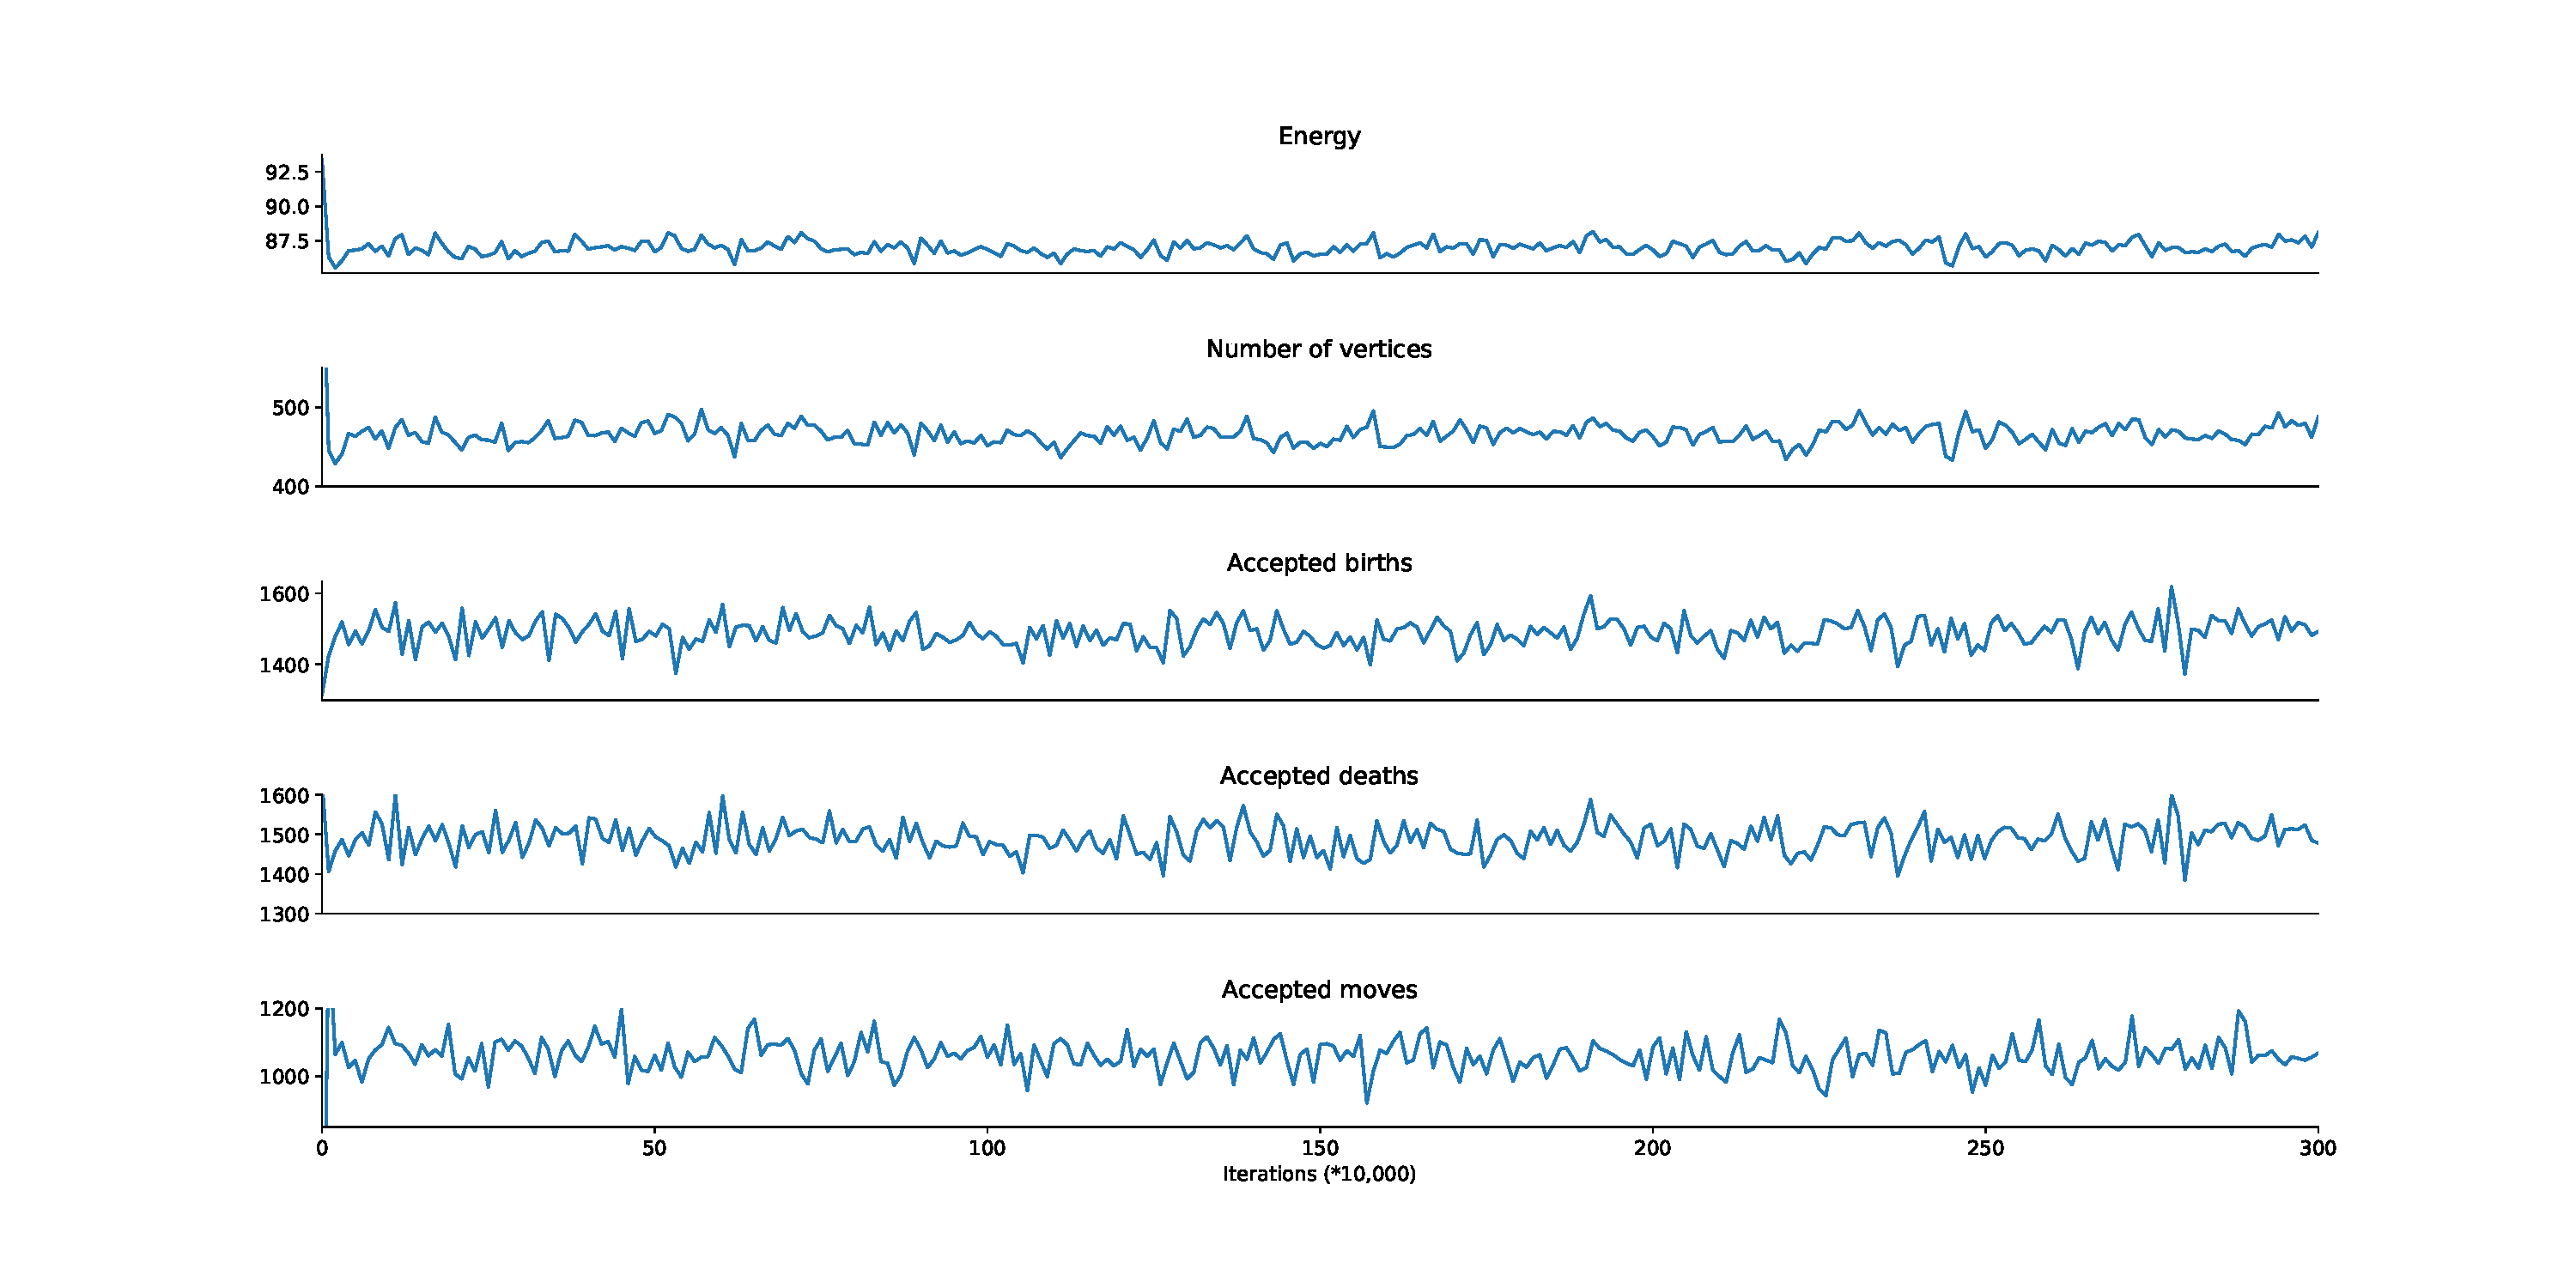
\includegraphics[width=1.3\textwidth]{../img/numeric/convergence.pdf}
  \caption{Convergence metrics for one simulation of \texttt{L+}. Total number of iterations: $3\times 10^6$. $\theta = 1, \alpha = 0.15, z = 500, W = 0.01$.}
  \label{fig:convergence}
\end{figure}




\subsection{Role of $\theta$}
The parameter $\theta$ plays an interesting role in our model. As noted before, the GPP favours configurations with lower energy. In case of the potential $\varphi^{\alpha,\theta}_{HC}$, this the configurations are forced to contain fewer larger tetrahedra in order to minimize the overall surface area. The parameter $\theta$ then controls the strength of this effect. Higher $\theta$ should therefore result in a smaller number of larger tetrahedra. This effect can be seen in Figure \ref{fig:thetaeffect} for one realization of the model $L+$.

\begin{figure}
  \centering
  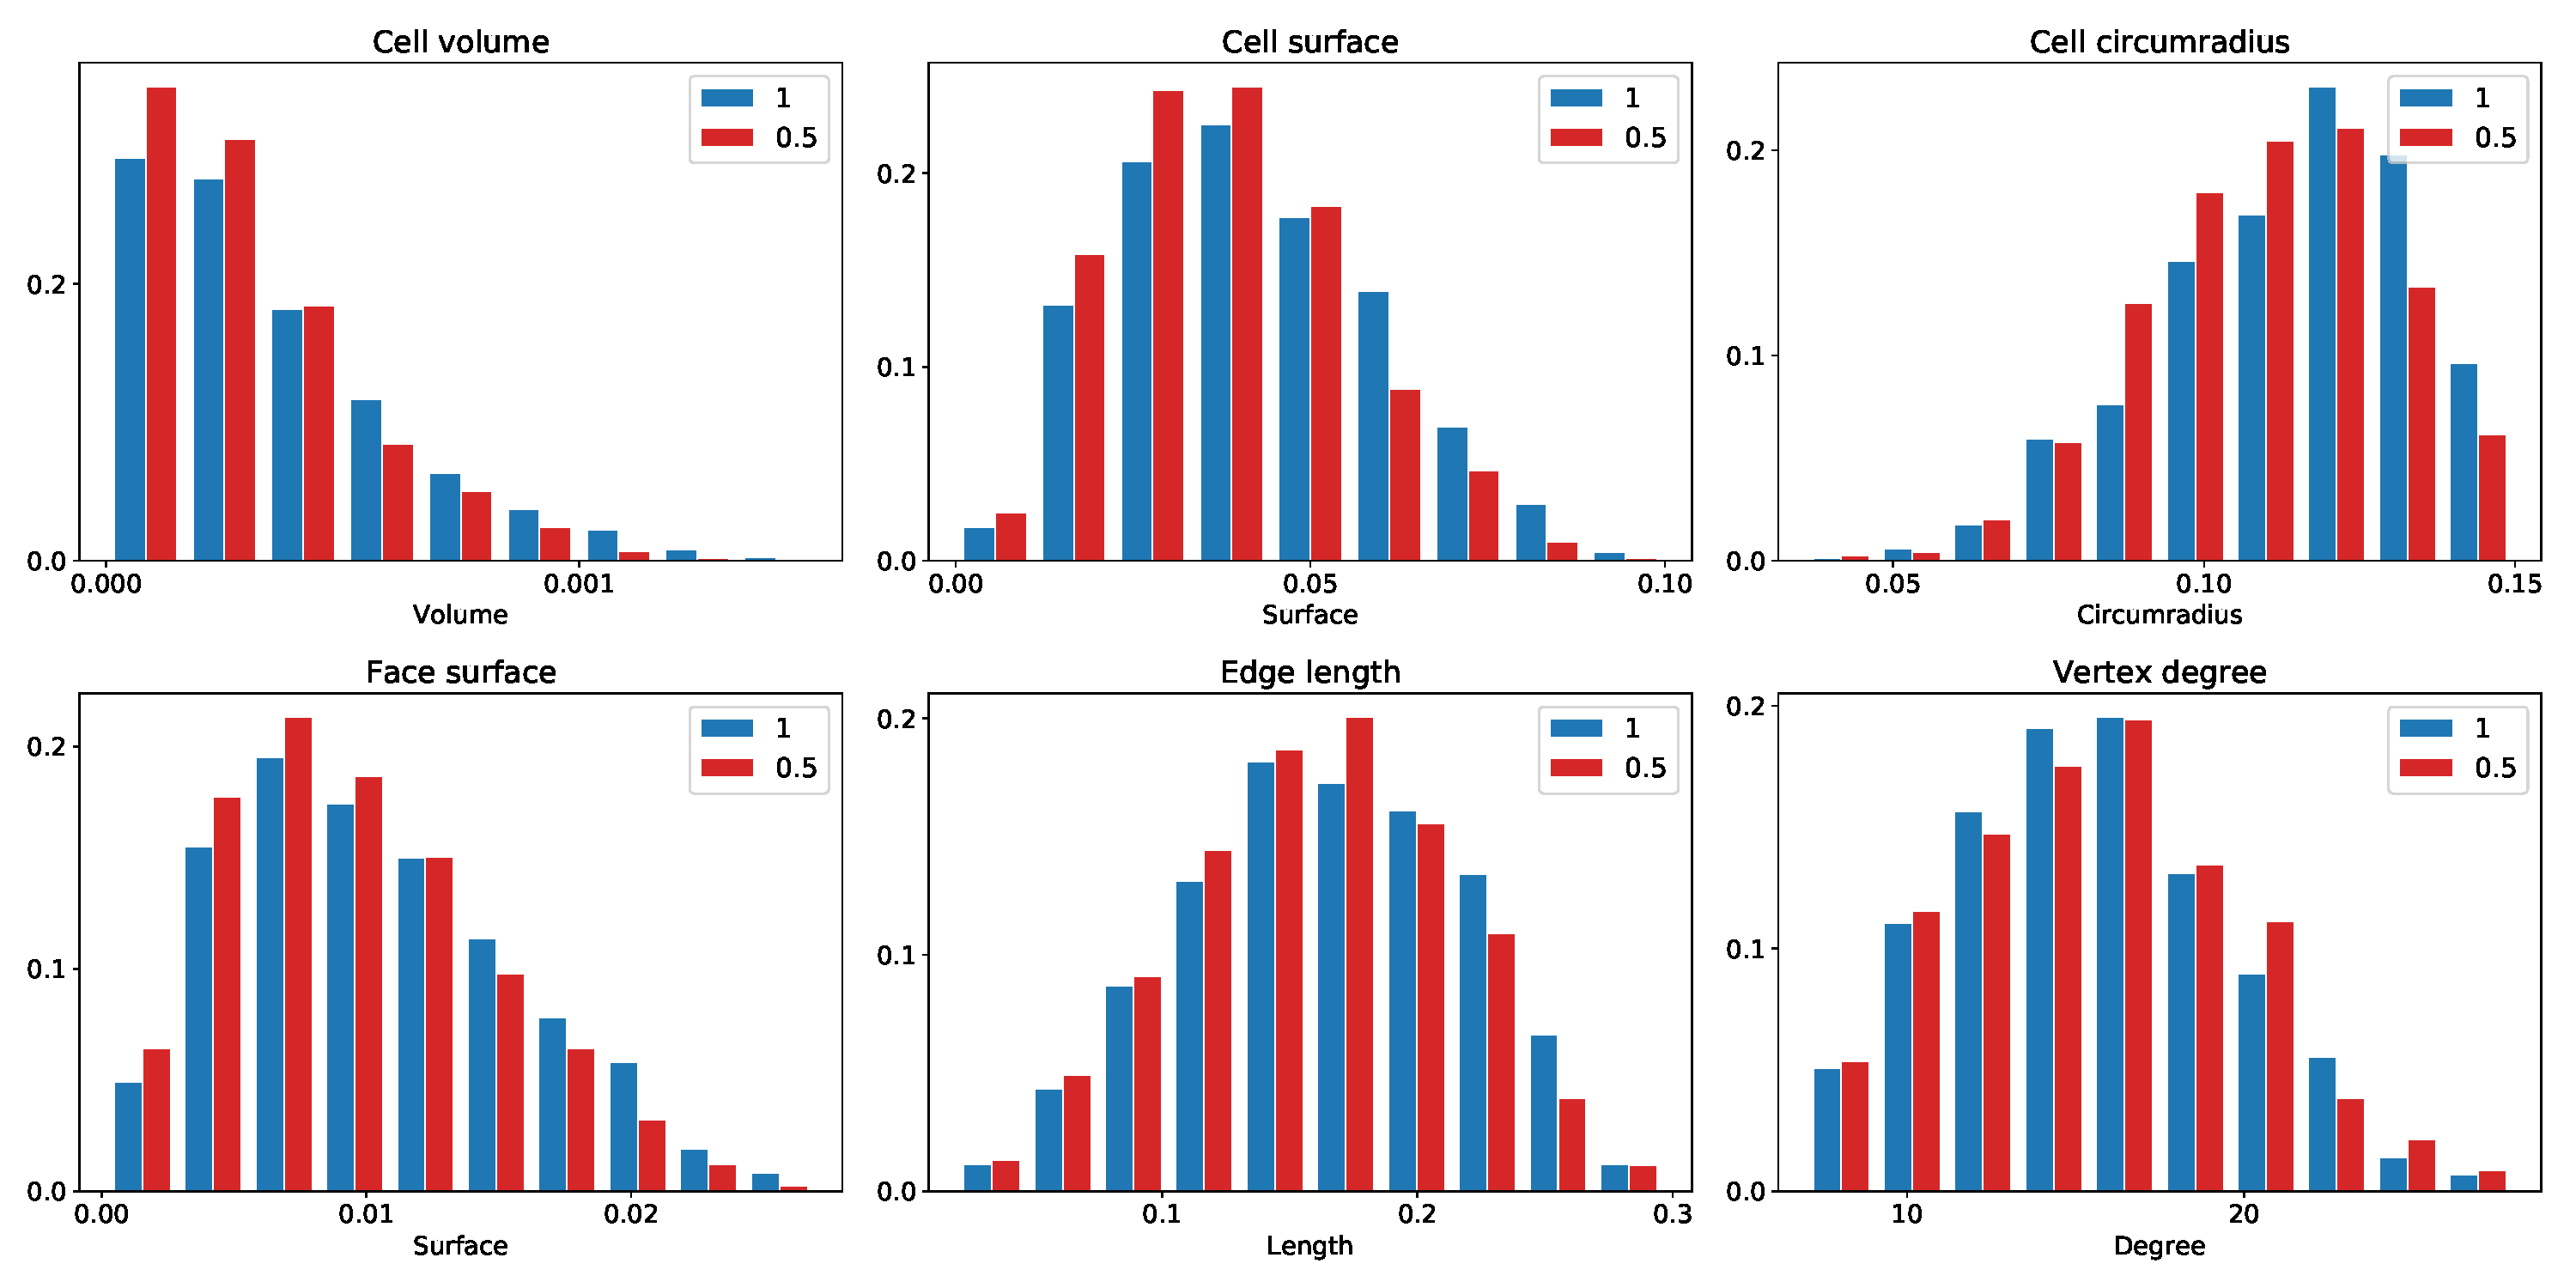
\includegraphics[width=1\textwidth]{../img/numeric/facets_1_05.pdf}
  \caption{Comparison of the distribution of facet statistics for one realization of \texttt{L+} model with $\alpha=0.15,z=500,W=0.01$ and $\theta = 0.5,1$.  }
  \label{fig:thetaeffect}
\end{figure}


Although we have restricted ourselves to the case of non-negative potentials, it is still interesting to attempt to simulate models with a $\theta<0$, even if we do not know whether they exist. Choosing $\theta$ negative reverses the relationship mentioned above. The GPP now favours configurations with greater overall surface area, which should result into a larger number of smaller tetrahedra. This is in fact what happens in the simulation, see Figure \ref{fig:thetanegative}.


% Plot theta pos neg
\begin{figure}
  \centering
    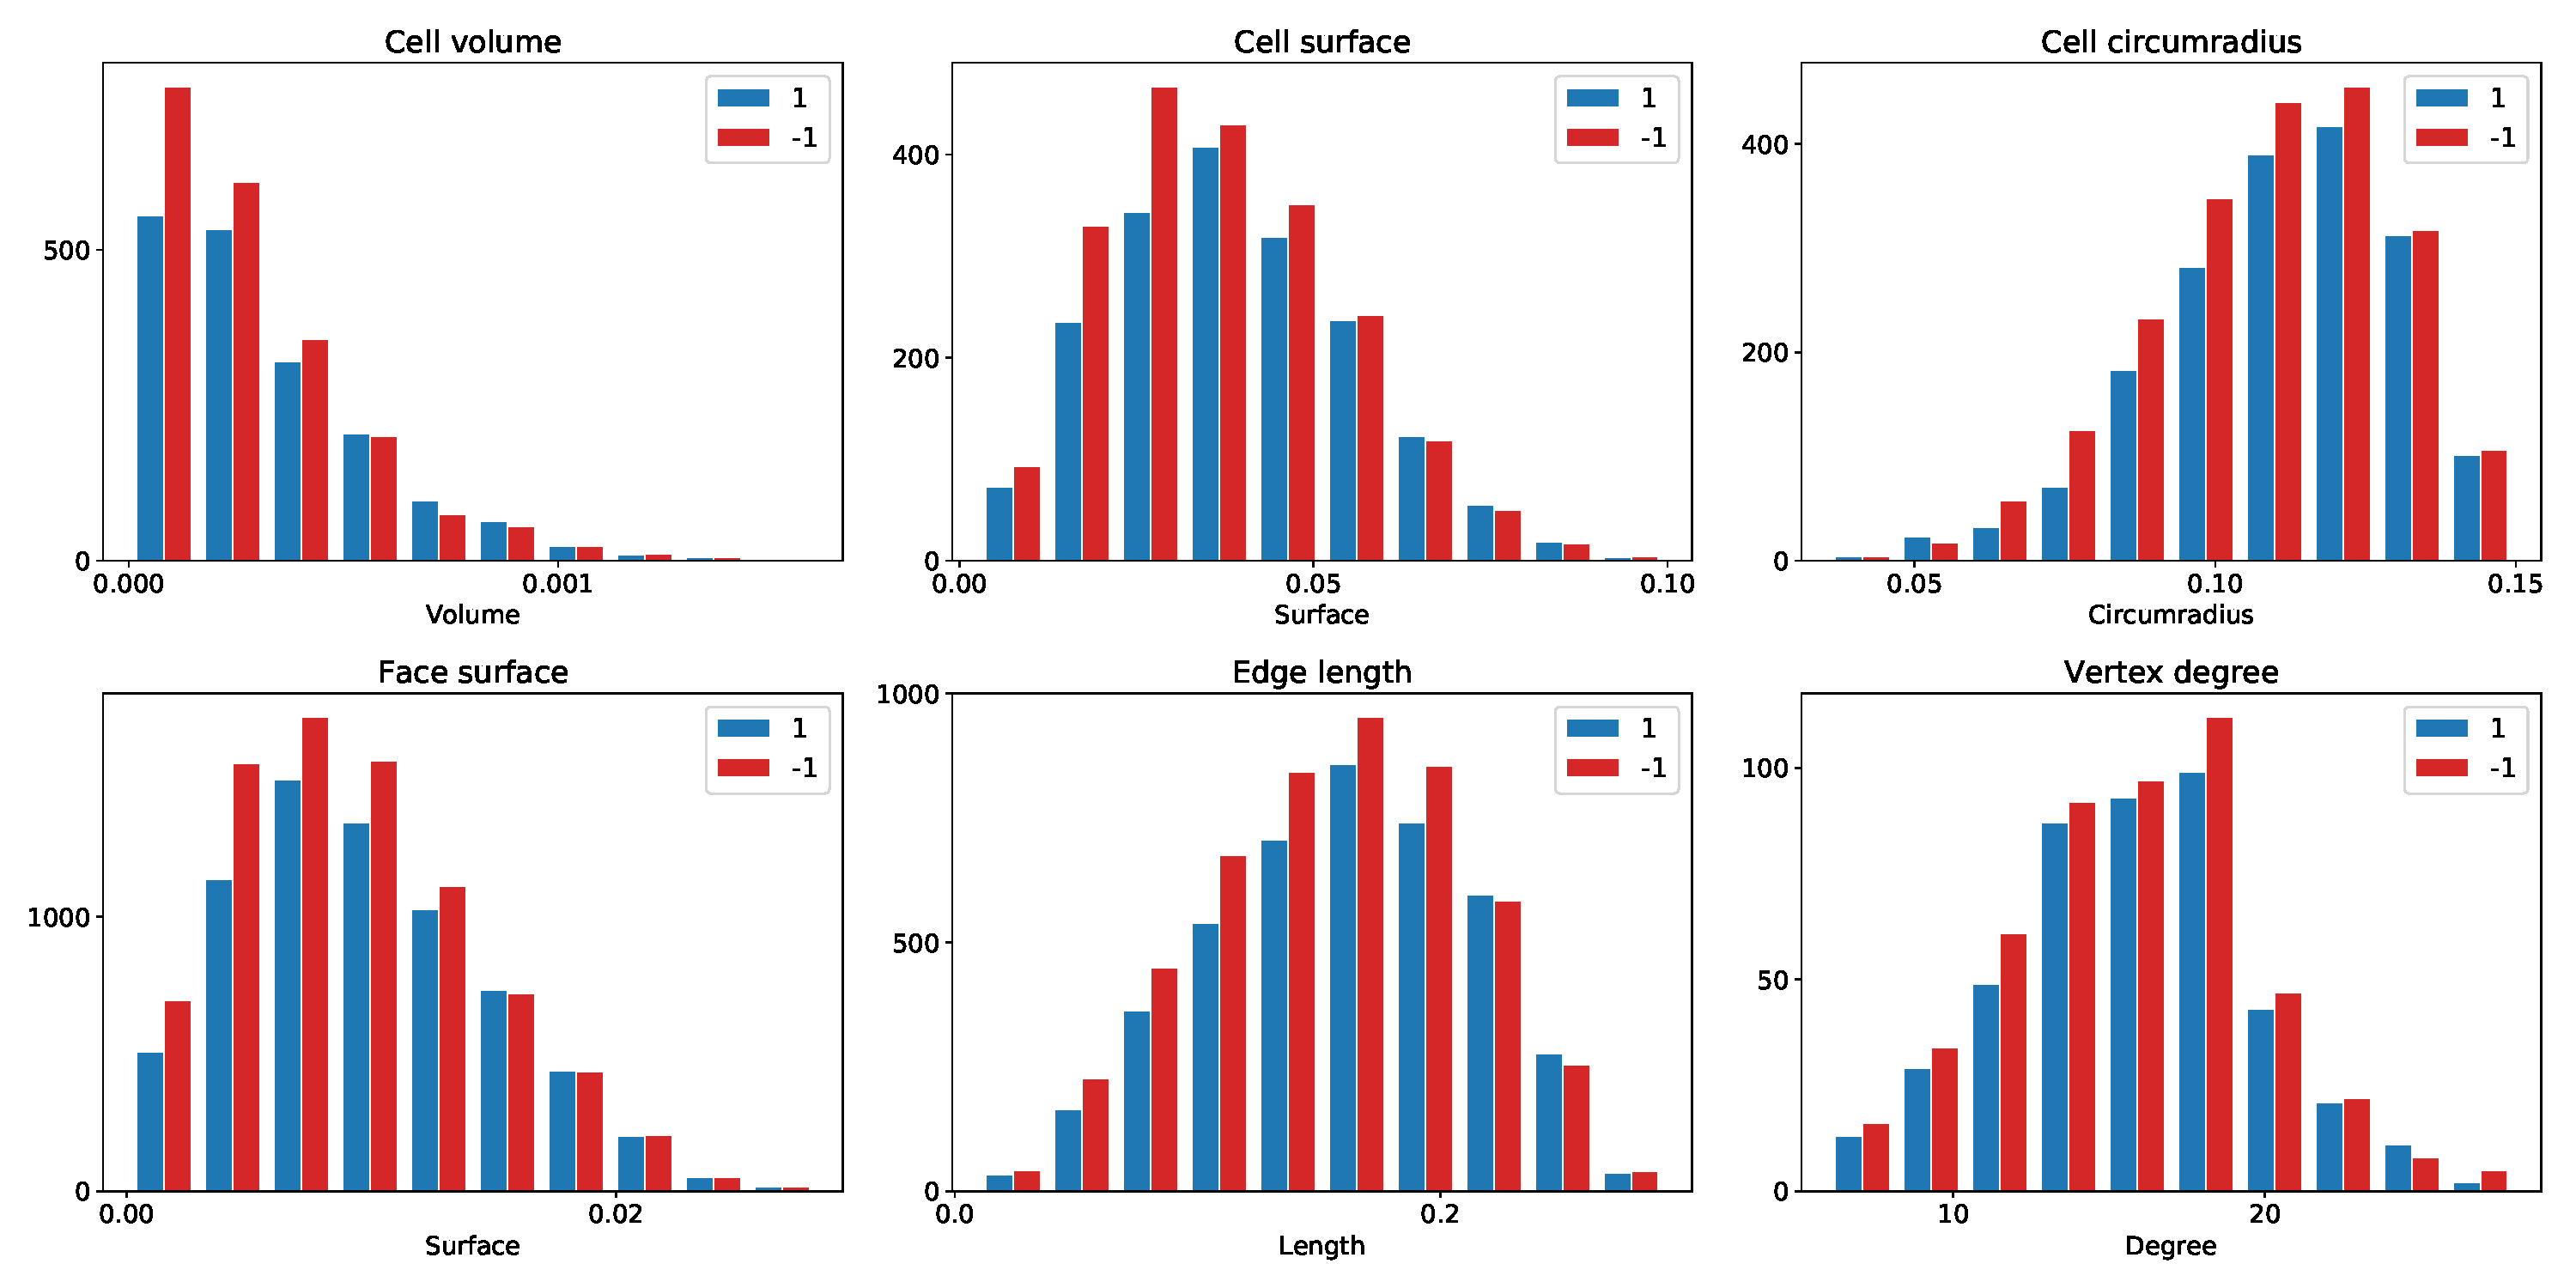
\includegraphics[width=1\textwidth]{../img/numeric/facets_1_-1.pdf}
  \caption{Comparison of the distribution of facet statistics for one realization of \texttt{L+} model with $\alpha=0.15,z=500,W=0.01$ and $\theta = -1,1$.  }
  \label{fig:thetanegative}
\end{figure}




\subsubsection{Obtaining the Poisson tetrahedrization}
\todoo[inline]{This should possibly be shown already in Ch 2 and only referenced here}
From Proposition \ref{prop:poisabscont}, we know that for $\Lambda \in \mathcal B_0(\Rt)$, the Poisson point process with intensity $z$ has the density $f(\gamma)\propto z^{N_\Lambda}(\gamma), \gamma \in \mathbf N_\Lambda$  with respect to $\Pi_\Lambda$. From Definition \ref{def:GPP} of the Gibbs point process we can deduce that if the energy function is zero for all configurations, then the Gibbs point process with activity $z$ reduces to the Poisson point process with intensity $z$.  Figure \ref{fig:PoisvsGibbs} illustrates this point, where the facet distributions of a realization of the model \texttt{L+} with $\theta=0.01$ are compared to the expected values of their counterparts for the Poisson process (found on page $393$ in \cite{Okabe1992}).

% Plot theta 0.01 with Poisson theoretic
\begin{figure}
  \centering
    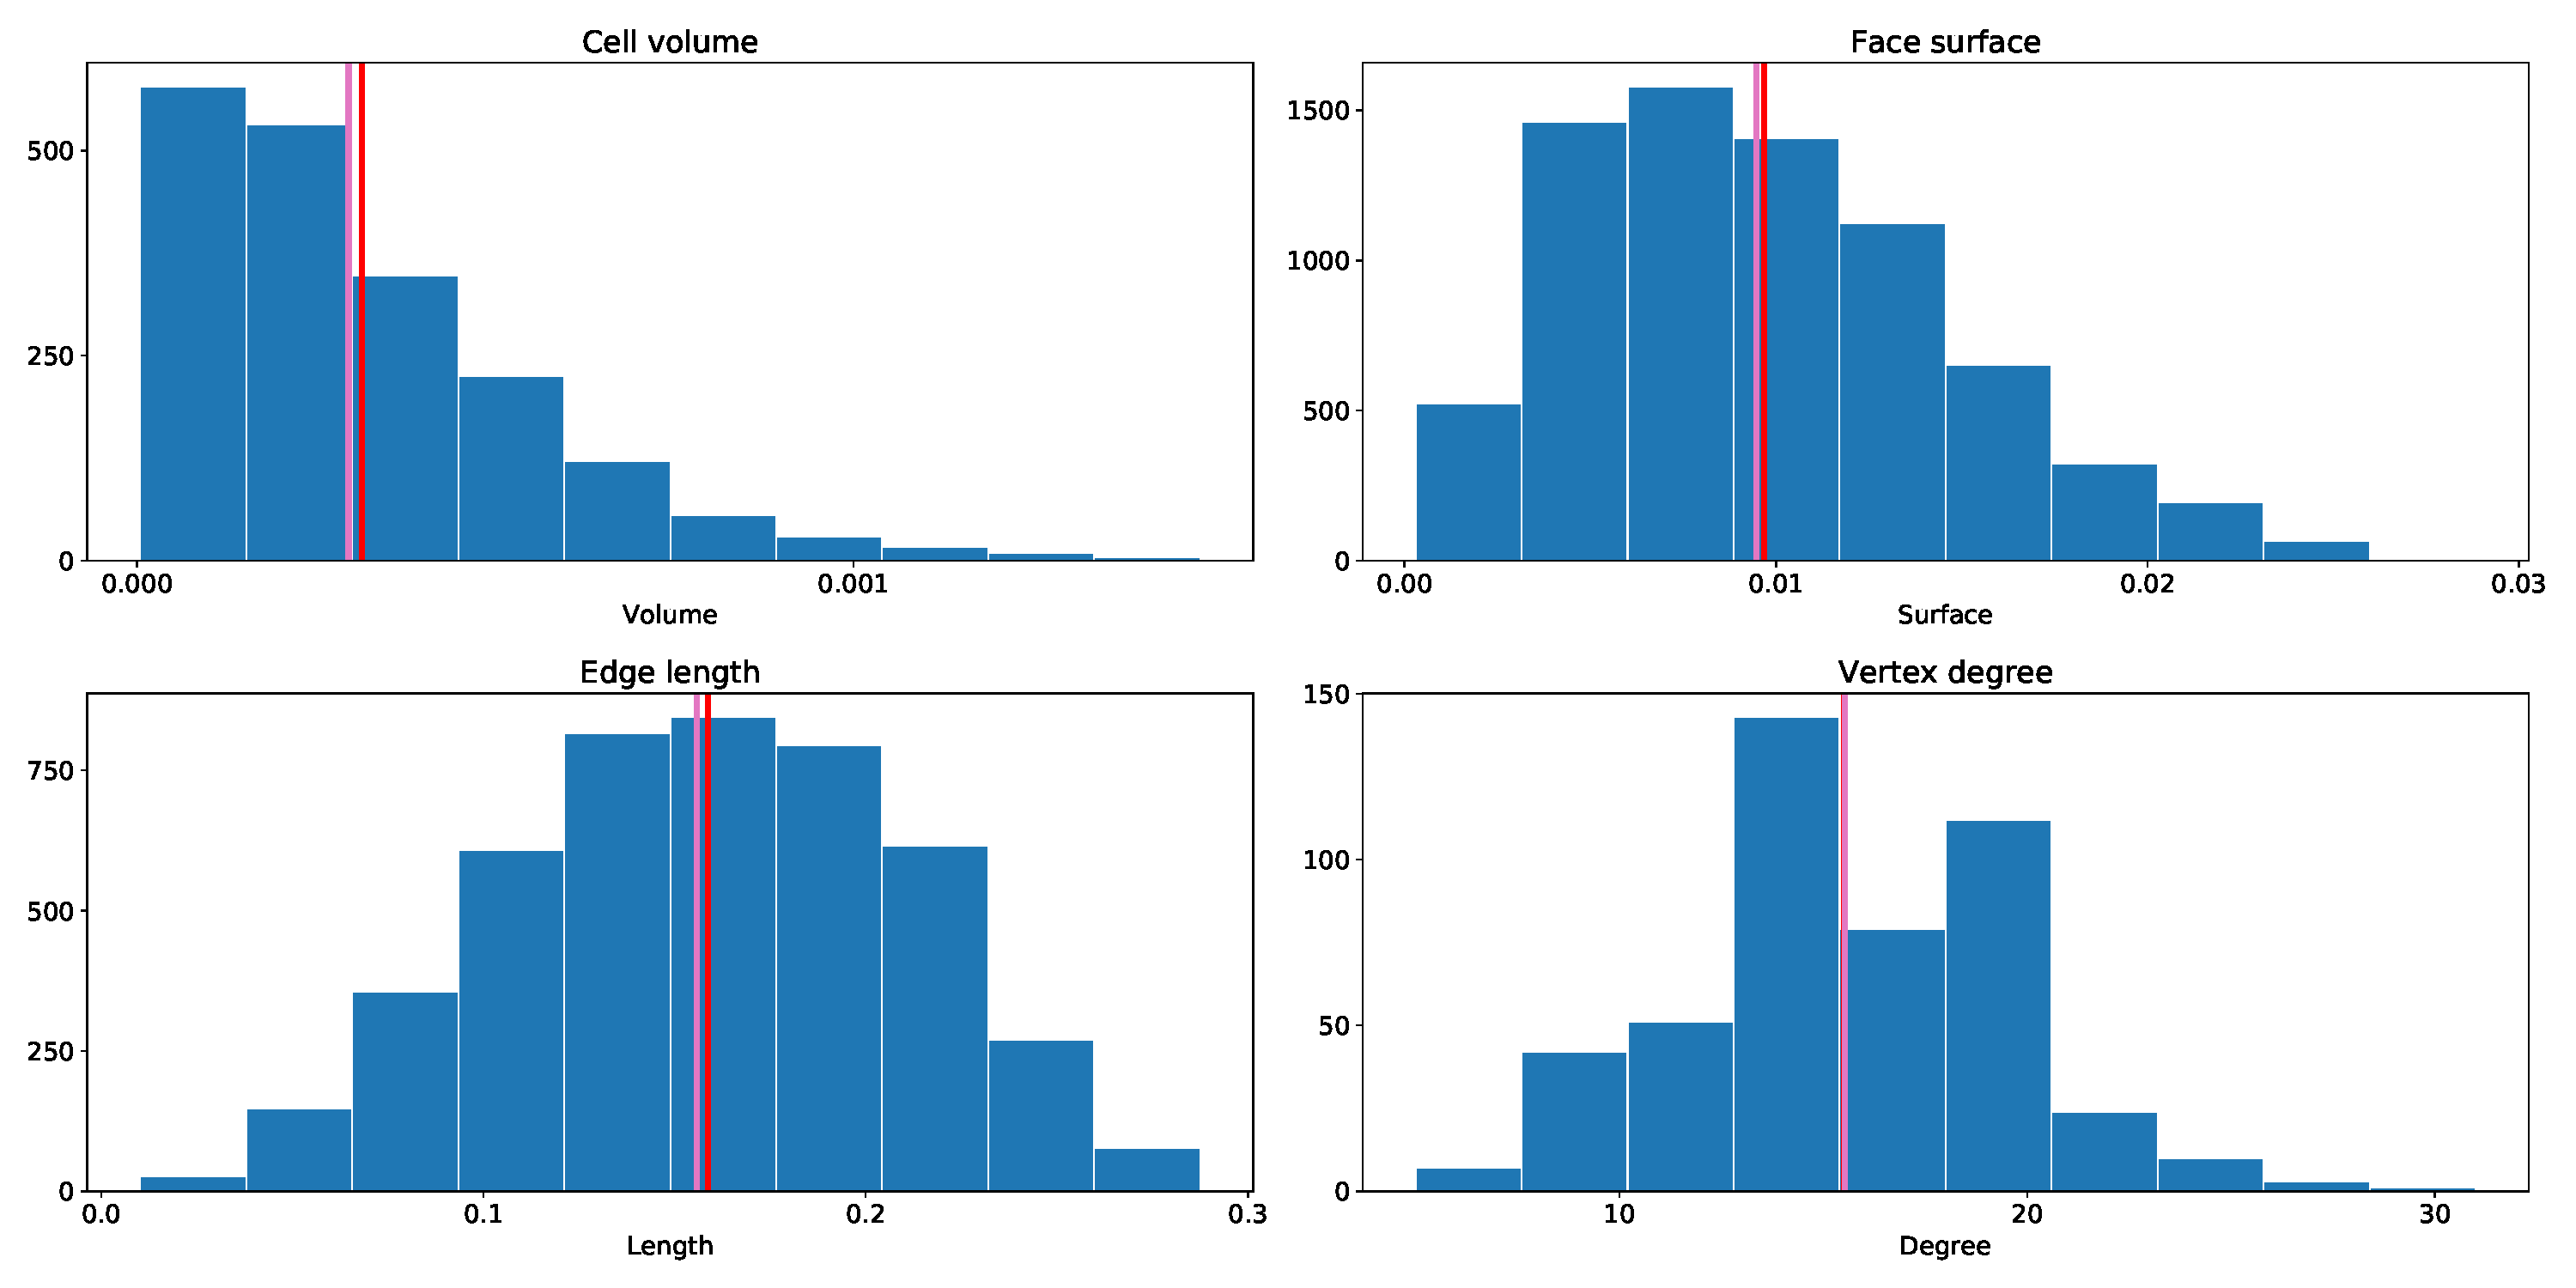
\includegraphics[width=1\textwidth]{../img/numeric/poisson.pdf}
  \caption{Facet distributions of a realization of the \texttt{L+} model with $\alpha=0.15,z=500,W=0.01$ and $\theta = 0.01$. Purple line is the expected value for a Poisson-tetrahedrization, red line is the empirical mean of the realization.  }
  \label{fig:PoisvsGibbs}
\end{figure}




\subsection{Difference between Laguerre and Delaunay}
Perhaps the most interesting comparison to make is between the two models \texttt{D+} and \texttt{L+} with identical parameters. A summary of facet distributions for a realization of both models is shown in Figure  \ref{fig:DelvsLag}.
\todoo[inline]{comment more}

% Plot model differences 

\begin{figure}
  \centering
    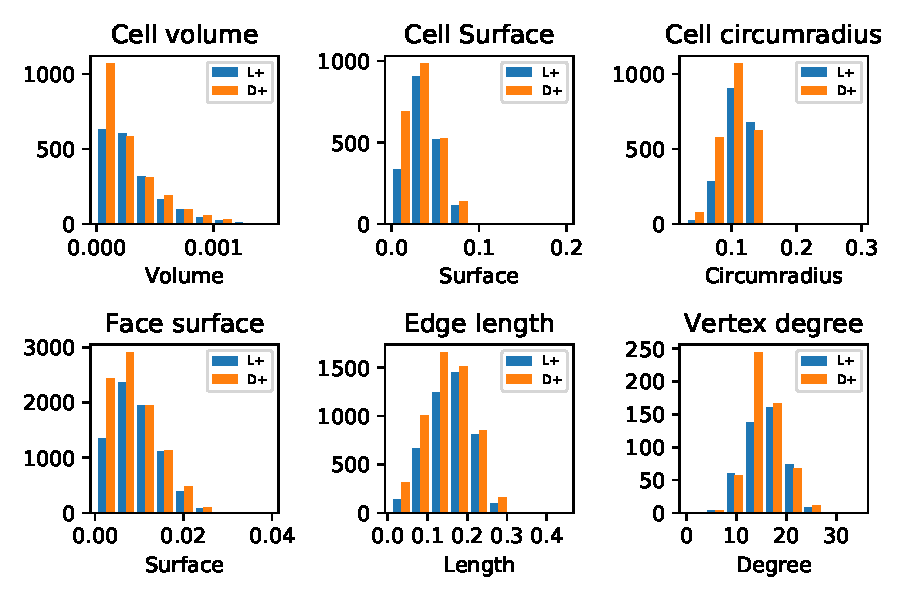
\includegraphics[width=1\textwidth]{../img/numeric/facets_L+_D+.pdf}
  \caption{Facet distribution for a realization of the models \texttt{D+} and \texttt{L+}. Parameters $\theta = 1,\alpha = 0.15, z=500, W=0.01$ for both models.}
  \label{fig:DelvsLag}
\end{figure}


All of the results for both \texttt{D+} and \texttt{L+} with four $\theta$ levels are summarized in Table \ref{tab:facets}, which shows the averages and standard deviations for a $100$ simulations of each model.


\begin{landscape}
\begin{table*}\centering
\ra{1.3}
\begin{tabular}{lrllllllll}\toprule
&& \multicolumn{4}{c}{Cell} & \multicolumn{1}{c}{Face} & \multicolumn{1}{c}{Edge} & \multicolumn{2}{c}{Vertex} \\ 
\cmidrule(lr){3-6} \cmidrule(lr){7-7} \cmidrule(lr){8-8} \cmidrule(lr){9-10}
& Theta &  Count & Volume & Circumradius & Surface & Surface & Length & Count & Degree \\
\midrule
\texttt{D+} \\
 & -1.0 &  2761.3 &  0.00023 &  0.1011 &  0.0322 &  0.0081 &  0.1453 &  639.6 &  15.4 \\
 & &  (108.1) &  (0.00001) &  (0.0012) &  (0.0008) &  (0.0002) &  (0.0017) &  (20.0) &  (0.1) \\
 & -0.5 &  2685.7 &  0.00024 &  0.1015 &  0.0326 &  0.0082 &  0.1461 &  626.2 &  15.4 \\
 & &  (119.9) &  (0.00001) &  (0.0016) &  (0.0010) &  (0.0003) &  (0.0024) &  (22.5) &  (0.1) \\
 & 0.5 &  2509.0 &  0.00025 &  0.1028 &  0.0337 &  0.0085 &  0.1481 &  595.2 &  15.4 \\
 & &  (103.3) &  (0.00001) &  (0.0014) &  (0.0009) &  (0.0002) &  (0.0020) &  (19.0) &  (0.1) \\
 & 1.0 &  2416.4 &  0.00026 &  0.1036 &  0.0344 &  0.0086 &  0.1495 &  577.3 &  15.4 \\
 & &  (100.9) &  (0.00001) &  (0.0013) &  (0.0009) &  (0.0002) &  (0.0018) &  (19.3) &  (0.1) \\
\texttt{L+} \\
 & -1.0 &  2082.9 &  0.00030 &  0.1090 &  0.0373 &  0.0094 &  0.1565 &  496.7 &  15.5 \\
 & &  (81.4) &  (0.00001) &  (0.0013) &  (0.0010) &  (0.0003) &  (0.0020) &  (16.5) &  (0.1) \\
 & -0.5 &  2022.4 &  0.00030 &  0.1096 &  0.0378 &  0.0095 &  0.1574 &  484.4 &  15.5 \\
 & &  (92.7) &  (0.00001) &  (0.0012) &  (0.0009) &  (0.0002) &  (0.0019) &  (18.0) &  (0.1) \\
 & 0.5 &  1909.3 &  0.00032 &  0.1105 &  0.0388 &  0.0097 &  0.1593 &  460.8 &  15.6 \\
 & &  (84.8) &  (0.00002) &  (0.0015) &  (0.0012) &  (0.0003) &  (0.0024) &  (16.1) &  (0.1) \\
 & 1.0 &  1855.3 &  0.00033 &  0.1110 &  0.0394 &  0.0099 &  0.1603 &  451.9 &  15.6 \\
 & &  (86.7) &  (0.00001) &  (0.0013) &  (0.0011) &  (0.0003) &  (0.0020) &  (16.3) &  (0.1) \\
\bottomrule
\end{tabular}
\caption{Facet statistics computed from $100$ realizations of each model and $\theta$ setting. Other parameters were set to $\alpha=0.15, z=500, W=0.01$.}
\label{tab:facets}
\end{table*}
\todoo[inline]{Write more, repeat first row, also std}
\end{landscape}





\section{Estimation}
% Estimation results (table+plot) for a few models
This section presents the results of the estimation procedure presented in Chapter \ref{ch:estimation}. Figures \ref{fig:estD05}, \ref{fig:estD1}, \ref{fig:estL05}, and \ref{fig:estL1} each show the results for the models \texttt{D+} and \texttt{L+}  with $\theta$ equal to $0.5$ and $1$. The bottom-right plot in each figure suggests a linear relationship between the estimates $\hat\theta$ and $\hat z$, a relationship that can be seen in the results of \cite{DereudreLavancier2011} as well.
\todoo[inline]{Comment on the badness, add reference to Dereudre}
Table \ref{tab:estsummary} summarizes all estimation results. 


\begin{table*}
\ra{1.3}
\resizebox{\textwidth}{!}{
\begin{tabular}{lrlllllll}\toprule
&& \multicolumn{1}{c}{$\hat\alpha$}& \multicolumn{2}{c}{$\hat\theta$} & \multicolumn{2}{c}{$\hat z$} & \multicolumn{2}{c}{Vertices} \\ 
 \cmidrule(lr){4-5} \cmidrule(lr){6-7} \cmidrule(lr){8-9} 

& $\theta$ &  &  $z$ unknown & $z$ known & $\theta$ unknown & $\theta$ known & All & Removable  \\
\midrule
\texttt{D+} \\
 & 0.5 &  0.14933 &  1.16643 &  0.22831 &  595.83387 &  564.27343 &  595.24 &  538.37 \\
 &  &  (0.00069) &  (0.94777) &  (0.56386) &  (52.15171) &  (23.55674) &  (18.98) &  (23.18) \\
 & 1.0 &  0.14946 &  1.84958 &  0.83162 &  605.18565 &  564.66566 &  577.32 &  515.81 \\
 &  &  (0.00050) &  (1.03663) &  (0.62494) &  (58.29123) &  (25.83548) &  (19.28) &  (24.94) \\
\texttt{L+} \\
 & 0.5 &  0.15455 &  1.20596 &  4.06347 &  306.40235 &  285.50261 &  460.83 &  269.36 \\
 &  &  (0.02235) &  (1.44752) &  (0.84692) &  (41.40474) &  (16.00663) &  (16.13) &  (15.71) \\
 & 1.0 &  0.15580 &  1.71939 &  4.49746 &  312.60278 &  290.65149 &  451.88 &  261.60 \\
 &  &  (0.04506) &  (1.41497) &  (0.76320) &  (46.78521) &  (18.69764) &  (16.31) &  (17.60) \\
\bottomrule
\end{tabular}}
\caption{Estimation summary. Each $\theta$ was simulated $100$ times. Parameters $\alpha=0.15,z=500, W=0.01$. }
\label{tab:estsummary}
\end{table*}





\begin{figure}
  \centering
  \includegraphics[width=1\textwidth]{"../img/numeric/estimation - type_D+_theta_05"}
  \caption{Estimation results for the model \texttt{D+} with parameters $\theta=0.5,z=500,W=0.01$ for 100 realizations.}
  \label{fig:estD05}
\end{figure}


\begin{figure}
  \centering
  \includegraphics[width=1\textwidth]{"../img/numeric/estimation - type_D+_theta_1"}
  \caption{Estimation results for the model \texttt{D+} with parameters $\theta=1,\alpha=0.15,z=500,W=0.01$ for 100 realizations. Average number of removable points: $442$.}
  \label{fig:estD1}
\end{figure}

\begin{figure}
  \centering
  \includegraphics[width=1\textwidth]{"../img/numeric/estimation - type_L+_theta_05"}
  \caption{Estimation results for the model \texttt{L+} with parameters $\theta=0.5,z=500,W=0.01$ for 100 realizations. }
  \label{fig:estL05}
\end{figure}


\begin{figure}
  \centering
  \includegraphics[width=1\textwidth]{"../img/numeric/estimation - type_L+_theta_1"}
  \caption{Estimation results for the model \texttt{L+} with parameters $\theta=1,\alpha=0.15,z=500,W=0.01$ for 100 realizations. Average number of removable points: $261$.}
  \label{fig:estL1}
\end{figure}




